% Hazi Feladat / Meresi jegyzokony sablon BME MIT
% Keszult: 2012.13.17
% Leiras: Ebbe a fajlba kerul a lenyegi resz, a szoveg. A legfelsobb szintu felsorolas a section (chapter nem hasznalatos).

\section{A mérés bemutatása}
A mérésen játékelméleti problémák leírását, megoldását és szimulációját végeztük. Ehhez a GAMBIT játékleíró/megoldó szoftvert és JADEX es ágenseket használtunk.

\section{Otthoni feladat 1}
\subsection{Leírás}
A laborsegédlet és az egyéb segédanyagok maradéktalan elolvasását és megértését követően töltse le a labor weblapjáról (http://www.mit.bme.hu/oktatas/targyak/vimim223/feladat/4-Jatekelmelet) a labor forráskódjait és a GAMBIT (Software Tools for Game Theory) alkalmazást. Bontsa ki a forráskódokat a msclab01 könyvtárba, illetve telepítse a GAMBIT-et. Ezt követően nyissa meg, értelmezze, és oldja meg GAMBIT-tel a games könyvtárban található… 
a. pd.nfg
b. hd2v4.0c2.0.nfg
c. hd2v2.0c4.0.nfg
d. hd3v6.0c3.0.nfg
e. totc10.nfg


\subsection{Megoldás}
\begin{enumerate}
\item pd.nfg
		\begin{figure}[!h]
		\begin{center}
		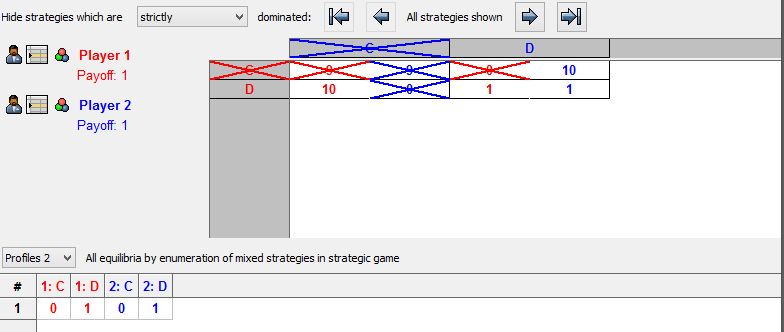
\includegraphics[height=7cm]{figures/pd_nfg_dom.png}
		\caption{A pd.nfg megoldása}
		\end{center}
		\end{figure}
A fogolydilemma szimmetrikus leírását tartalmazza, mint látható a domináns stratégia a ha egy ágens vall, és a Nash egyensúly az amikor mindketten vallanak.
		
\item hd2v4.0c2.0.nfg
		\begin{figure}[!h]
		\begin{center}
		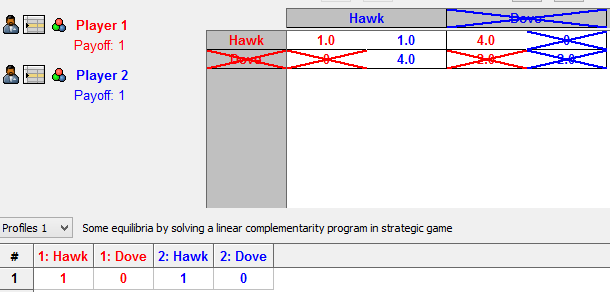
\includegraphics[height=7cm]{figures/hd2v4_dom.png}
		\caption{A hd2v4.0c2.0.nfg megoldása}
		\end{center}
		\end{figure}
A galamb-héja probléma egy olyan leírását tartalmazza, amelynek a domináns stratégiája a héja választás, ami egyben a Nash egyensúly is.
		
\item hd2v2.0c4.0.nfg
		\begin{figure}[!h]
		\begin{center}
		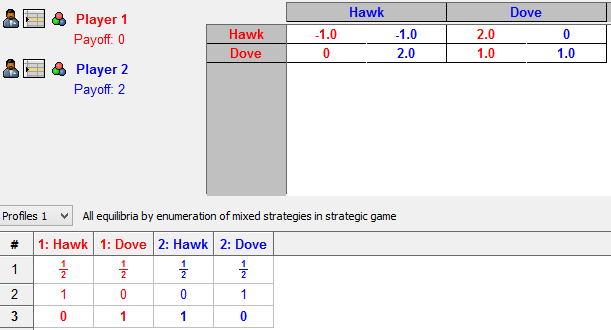
\includegraphics[height=7cm]{figures/hd2v2.png}
		\caption{A hd2v2.0c4.0.nfg megoldása}
		\end{center}
		\end{figure}
A galamb-héja probléma egy olyan leírását tartalmazza, amelynek nincsen domináns stratégiája, de van 3 Nash egyensúlya.
		
\item hd3v6.0c3.0.nfg
		\begin{figure}[!h]
		\begin{center}
		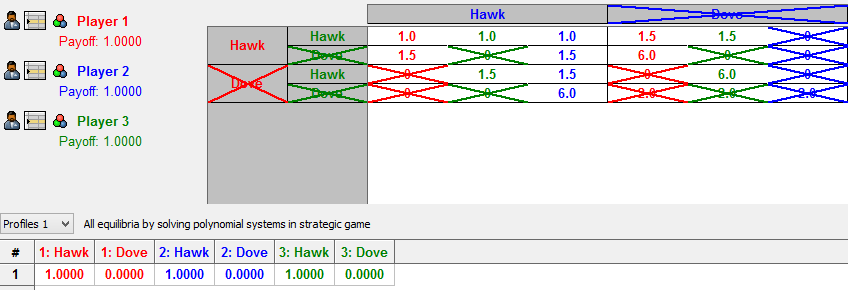
\includegraphics[height=5cm]{figures/hd3_dom.png}
		\caption{A hd3v6.0c3.0.nfg megoldása}
		\end{center}
		\end{figure}
A galamb-héja probléma 3 játékos változata, amiben a domináns stratégia a héja választás, a Nash egyensúly pedig akkor áll be, ha mindhárom játékos a héját választja.

\item totc10.nfg
		no dominance
		\begin{figure}[!h]
		\begin{center}
		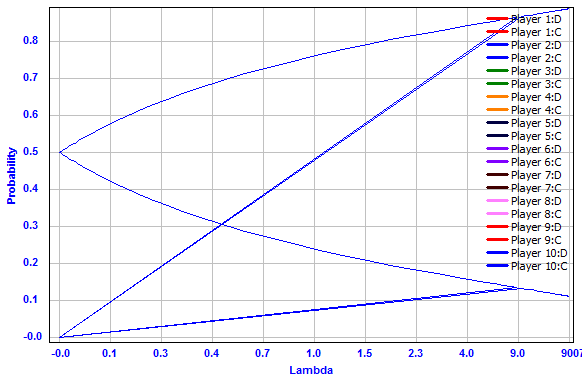
\includegraphics[height=7cm]{figures/tot.png}
		\caption{A totc10.nfg megoldása}
		\end{center}
		\end{figure}
A közös legelő problémát írja le 10 játékos esetén. Nem rendelkezik domináns stratégiával, sem Nash egyensúlyal.
		
\end{enumerate}
\section{Otthoni feladat 2}
\subsection{Leírás}
A GAMBIT segítségével… a. …építse fel alapvető játékok (Fogolydilemma, Gyáva nyúl, Nemek harca, Vezérürü, Érmepárosítás, Közlegelők tragédiája, 2-lapos póker, stb) extenzív és/vagy normál alakját majd pedig elemezze az elkészült játékokat (találja meg bennük a domináns stratégiákat, illetve a Nash-egyensúlyokat)! b. Az elkészült játékok normál alakját mentse el a games könyvtárba új fájlnevekkel, és egészítse ki őket egy-egy megfelelő .nfo fájllal! Minta gyanánt használhatja a pd.nfo fájlt. Lényegében tehát egy azonos nevű, .nfo kiterjesztésű szövegfájlt (meta-információt) kell létrehoznia minden egyes előbb létrehozott és mentett normál-formájú játék mellé. Ez egy tab-delimited szövegfájl legyen, aminek első eleme (0 vagy 1) adja meg, hogy a kapcsolódó játék szimmetrikus-e, második eleme (0 vagy 1) azt mondja meg, hogy van-e ebben a játékban minden játékosnak ún. kooperatív tiszta stratégiája, és amennyiben ez igaz, úgy harmadik eleme az egyes játékosok kooperatív tiszta stratégia-azonosítóinak (0, 1, 2, …) szóközökkel elválasztott listája, ahol a játékosok sorrendje a kapcsolódó .nfg fájlban megadott sorrendnek feleljen meg.

\subsection{Megoldás}
A segédletben leírtak szerint felépítettem a következő problémák normál alakját, és megoldottam őket.
\begin{itemize}
\item Fogolydilemma
		\begin{figure}[!h]
		\begin{center}
		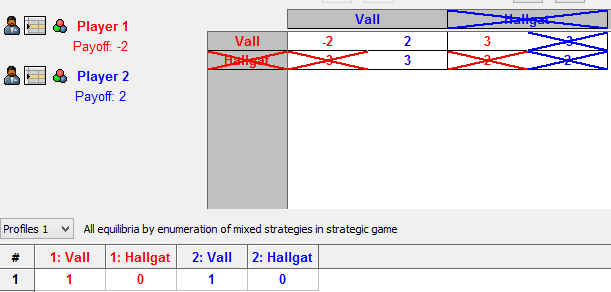
\includegraphics[height=7cm]{figures/fogoly.png}
		\caption{A fogolydilemma megoldása}
		\end{center}
		\end{figure}
Amint láthat a fogolydilemma ezen formájának a domináns stratégiája a vall, és a Nash egyensúlya amikor mindkét fogoly vall. A játék szimmetrikus, ennek értelmében az nfo fájl tartalma:1	1	1 1.
		
\item Gyáva nyúl
		\begin{figure}[!h]
		\begin{center}
		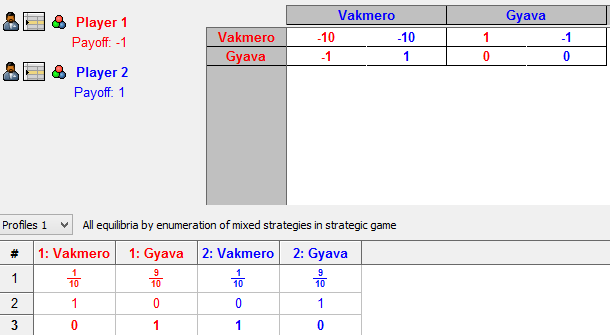
\includegraphics[height=7cm]{figures/nyul.png}
		\caption{A gyáva nyúl megoldása}
		\end{center}
		\end{figure}
A gyáva nyúl játéknak nincs domináns stratégiája, de van két Nash egyensúlya. A játék szimmetrikus, tehát az nfo fájl tartalma: 1	1	1 1
		
\item Nemek harca
		\begin{figure}[!h]
		\begin{center}
		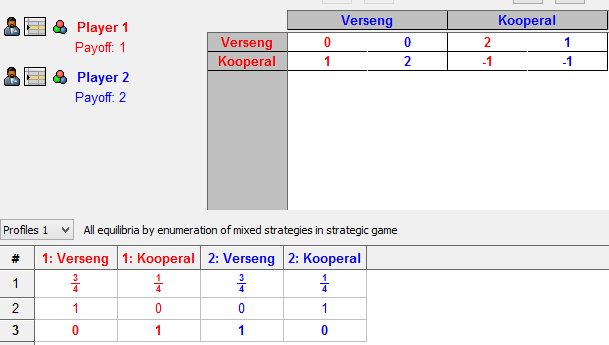
\includegraphics[height=7cm]{figures/nemek.png}
		\caption{A nemek harca megoldása}
		\end{center}
		\end{figure}
A nemek harcának ezen leírásában, nincs domináns stratégia, van 2 Nash egyensúly és a játék szimmetrikus. Az nfo fálj tehát:1	1	0 0
\item Vezérürü
		\begin{figure}[!h]
		\begin{center}
		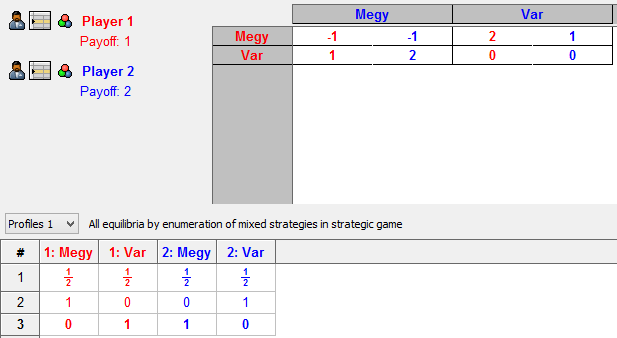
\includegraphics[height=7cm]{figures/uru.png}
		\caption{A vezérürü megoldása}
		\end{center}
		\end{figure}
A vezérürü játéknak nincs domináns stratégiájat, van 2 Nash egyensúlya és szimmetrikus. 
Az nfo fálj tehát:1	1	1 0
\item Érmepárosítás
		\begin{figure}[!h]
		\begin{center}
		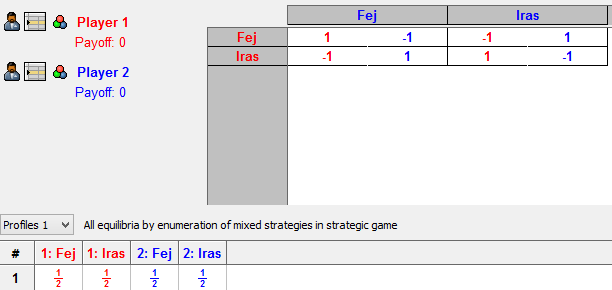
\includegraphics[height=7cm]{figures/erme.png}
		\caption{Az érmepárosítás megoldása}
		\end{center}
		\end{figure}
Az érmepárosítás játék asszimetrikus, nincs domináns stratégia és nincs Nash egyensúlya.
Az nfo fálj tehát:0	0
\end{itemize}

\section{Otthoni feladat 3}
\subsection{Leírás}
Futtassa az msclab01.gametheory-lab.Game osztályt az elkészült játékokkal (az osztály egyetlen argumentuma a normál-formájú játék fájlneve legyen kiterjesztés nélkül), és részletesen értelmezze a console kimenetet a 2/a feladatban látottak viszonylatában! Miket ír ki ez a program a konzolra? Minden adat helyes, amit kiír? Megjegyzés (FONTOS!!!): amennyiben egy eredetileg extenzív alakban létrehozott játékot normál formájú játékként exportálunk ki a GAMBIT-ből, de a Game osztály (vagy alább a GameAgent) nem hajlandó ezt rendesen beolvasni, úgy nyissuk meg külön ezt a kiexportált normál formájú játékot (.nfg fájlt) a GAMBIT-tel, és exportáljuk ki újra! Ennek hatására a kiexportált játék meg kell, hogy javuljon.  
\subsection{Megoldás}
A Game osztály beolvassa a problémát és meghatározza a játék Nash egyensúlyát.


\section{Otthoni feladat 4}
\subsection{Leírás}
Amennyiben megbizonyosodtunk arról, hogy az msclab01.gametheory-lab.Game osztály console kimenete helyes az általunk 2/a feladatban létrehozott összes játék esetén (vagy korrigáltuk az említett játékokat, és így lett helyes az output) Eclipse alól indítsunk el egy JADE platform-ot, majd pedig végezzünk egy-egy pár tucat körös tesztfuttatást mindegyik játék esetén! Magyarán minden játék kapcsán indítsuk el a szükséges számú felhasználói UserAgent és/vagy gépi Player ágenst (utóbbiaknak mindig legyen bekapcsolva a GUI-ja, és programjuk legyen a TFT), majd utána egy adott játékot host- oló GameAgent ágenst is, és regisztráljuk/dokumentáljuk a történteket! Mit látunk? Helyes a működés? …az egyes futtatásokhoz a segédletben látottaknak megfelelően Eclipse-es launch configuration-őket hozzunk létre (és ezeket is dokumentáljuk)! 
\subsection{Megoldás}
A jadex ágensek implementációja miatt átirtam a játékleírásokat egy olyan formára ami csak szigorúan pozítiv jutalmakat tartalmaz. Erre azért volt szükség, mert az ágensek leállnak ha <=0 a hasznuk.


		\begin{figure}[h]
		\begin{center}
		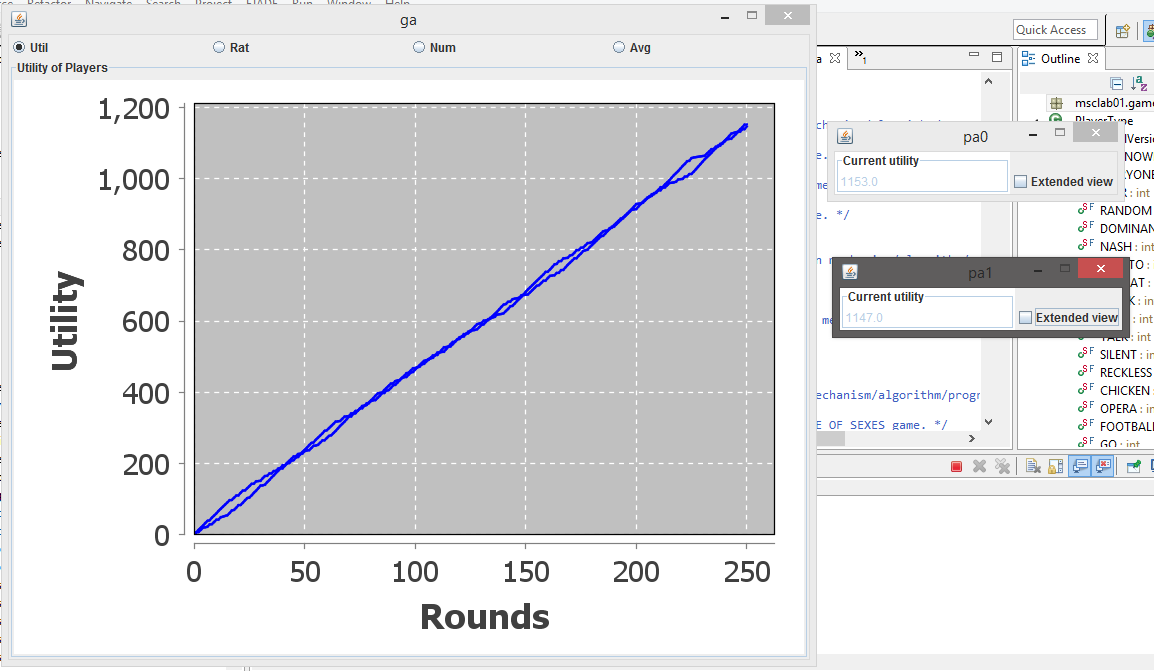
\includegraphics[height=7cm]{figures/fogoly_jadex.png}
		\caption{A fogolydilemma ágensekkel}
		\end{center}
		\end{figure}

\begin{lstlisting}[caption=Fogolydilemma run config, frame=single,float=!ht]
-container -port 1099 -host localhost 
ga:msclab01.gametheory_lab.GameAgent.GameAgent(fogolydilemma 2 2) 
pa0:jadex.adapter.jade.JadeAgentAdapter(msclab01.gametheory_lab.PlayerAgent.Player 
"default gid=\\\"fogolydilemma\\\" gui=true myType=7") 
pa1:jadex.adapter.jade.JadeAgentAdapter(msclab01.gametheory_lab.PlayerAgent.Player 
"default gid=\\\"fogolydilemma\\\" gui=true myType=7")
\end{lstlisting}
		

		\begin{figure}[h]
		\begin{center}
		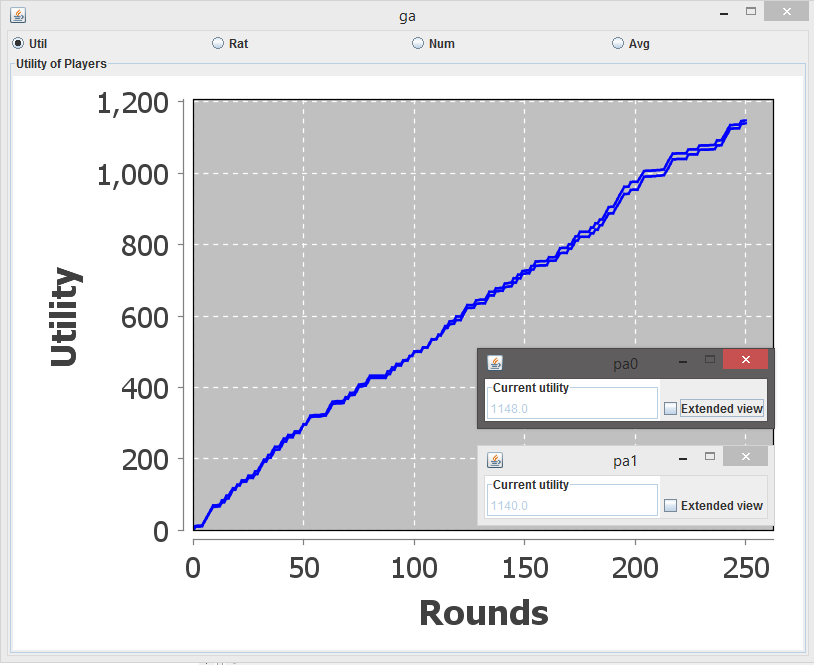
\includegraphics[height=7cm]{figures/nyul_jadex.png}
		\caption{A gyáva nyúl ágensekkel}
		\end{center}
		\end{figure}

\begin{lstlisting}[caption=Gyáva nyúl run config, frame=single,float=!ht]
-container -port 1099 -host localhost 
ga:msclab01.gametheory_lab.GameAgent.GameAgent(gyavanyul 2 2) 
pa0:jadex.adapter.jade.JadeAgentAdapter(msclab01.gametheory_lab.PlayerAgent.Player 
"default gid=\\\"gyavanyul\\\" gui=true myType=7") 
pa1:jadex.adapter.jade.JadeAgentAdapter(msclab01.gametheory_lab.PlayerAgent.Player 
"default gid=\\\"gyavanyul\\\" gui=true myType=7")
\end{lstlisting}
		

		\begin{figure}[h]
		\begin{center}
		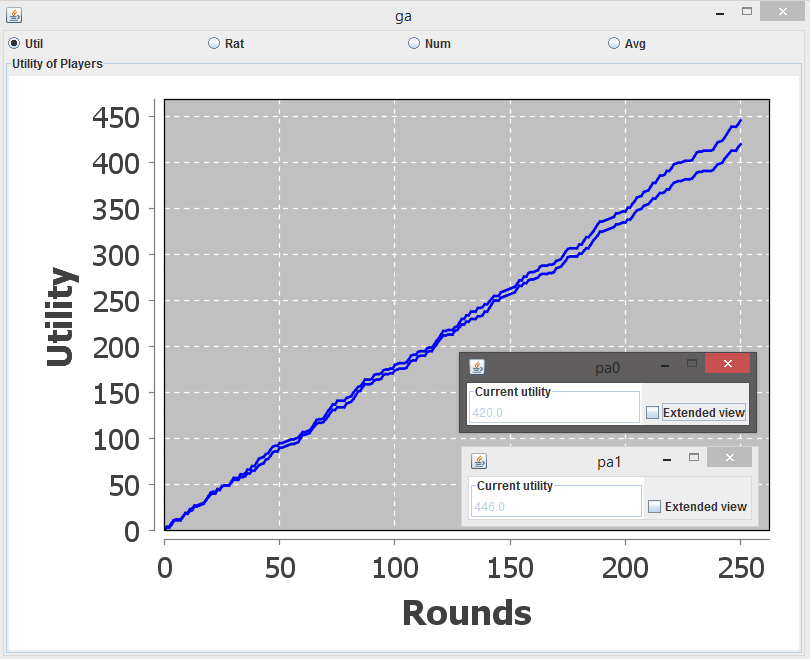
\includegraphics[height=7cm]{figures/nemek_jadex.png}
		\caption{A nemek harca ágensekkel}
		\end{center}
		\end{figure}

\begin{lstlisting}[caption=Nemek harca run config, frame=single,float=!ht]
-container -port 1099 -host localhost 
ga:msclab01.gametheory_lab.GameAgent.GameAgent(nemekharca 2 2) 
pa0:jadex.adapter.jade.JadeAgentAdapter(msclab01.gametheory_lab.PlayerAgent.Player 
"default gid=\\\"nemekharca\\\" gui=true myType=7") 
pa1:jadex.adapter.jade.JadeAgentAdapter(msclab01.gametheory_lab.PlayerAgent.Player 
"default gid=\\\"nemekharca\\\" gui=true myType=7")
\end{lstlisting}
		

		\begin{figure}[h]
		\begin{center}
		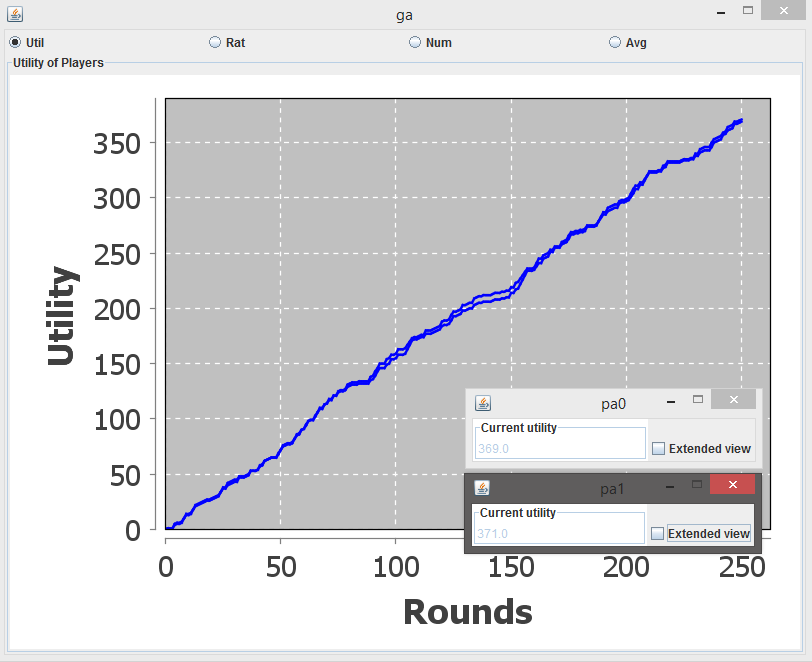
\includegraphics[height=7cm]{figures/uru_jadex.png}
		\caption{A vezérürü ágensekkel}
		\end{center}
		\end{figure}

\begin{lstlisting}[caption=Vezérürü run config, frame=single,float=!ht]
-container -port 1099 -host localhost 
ga:msclab01.gametheory_lab.GameAgent.GameAgent(vezeruru 2 2) 
pa0:jadex.adapter.jade.JadeAgentAdapter(msclab01.gametheory_lab.PlayerAgent.Player 
"default gid=\\\"vezeruru\\\" gui=true myType=7") 
pa1:jadex.adapter.jade.JadeAgentAdapter(msclab01.gametheory_lab.PlayerAgent.Player 
"default gid=\\\"vezeruru\\\" gui=true myType=7")
\end{lstlisting}
		

		\begin{figure}[h]
		\begin{center}
		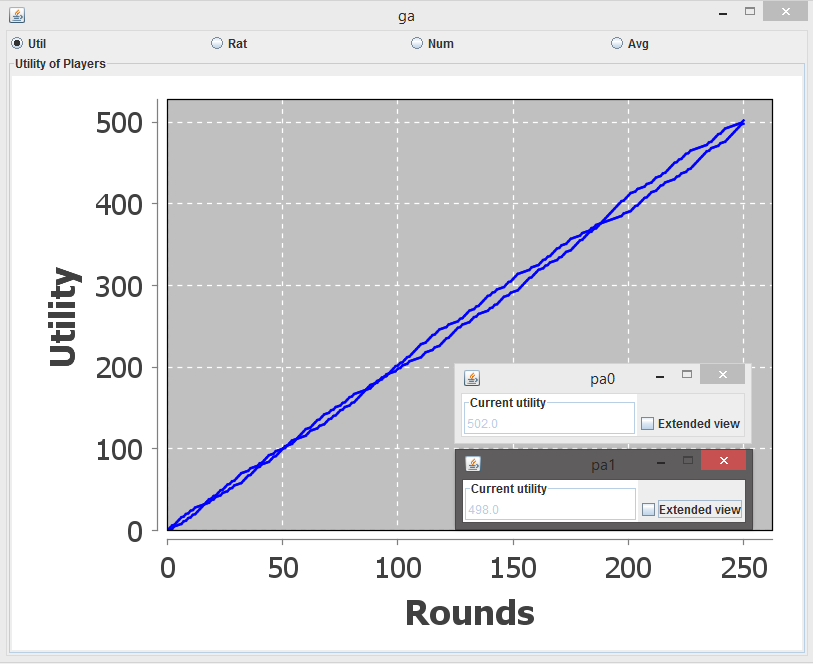
\includegraphics[height=7cm]{figures/erme_jadex.png}
		\caption{Az érmepárosítás ágensekkel}
		\end{center}
		\end{figure}

\begin{lstlisting}[caption=érmepárosítás run config, frame=single,float=!ht]
-container -port 1099 -host localhost 
ga:msclab01.gametheory_lab.GameAgent.GameAgent(ermeparositas 2 2) 
pa0:jadex.adapter.jade.JadeAgentAdapter(msclab01.gametheory_lab.PlayerAgent.Player 
"default gid=\\\"ermeparositas\\\" gui=true myType=7") 
pa1:jadex.adapter.jade.JadeAgentAdapter(msclab01.gametheory_lab.PlayerAgent.Player 
"default gid=\\\"ermeparositas\\\" gui=true myType=7")
\end{lstlisting}
		



\section{Labor feladat 1}
\subsection{Leírás}
Alakítsa ki GAMBIT-ben egy legalább 3 szereplős, legfeljebb néhány lépésből álló szavazás (pl. több fordulós (runoff) többségi szavazás) extenzív alakját, majd konvertálja ezt át normál alakba, elemezze, és mentse a games könyvtárba! Ellenőrizze az elkészült játékot az msclab01.gametheory-lab.Game osztály segítségével is! 
\subsection{Megoldás}
Az első lépésben egy két fordulós, többségi szavazást definiáltam a GAMBIT-ben, 3 játékossal és 3 jelöltel. Az ötlet az volt hogy csak akkor megy végbe a második forduló ha két játékos egy közös jelöltre szavazott, a harmadik pedig egy másikra. Ekkor az a jelölt akire senki sem szavazott kiesik és a játékosok preferencia listájuknak megfelelően újra szavaznak a bentmaradt jelöltekre. Ekkor akinek a legtöbb szavazata lett az a győztes. Az ágensek hasznát aszerint határoztam meg, hogy a győztes hol állt az adott ágens preferencia listáján. Ha minden játékos másra szavazott vagy ugyanarra, akkor nem volt újabb forduló. Az extenzív alak eléggé komplex lett, az egyszerű probléma ellenére is, mint az ábra mutatja.
\begin{figure}[h]
\begin{center}
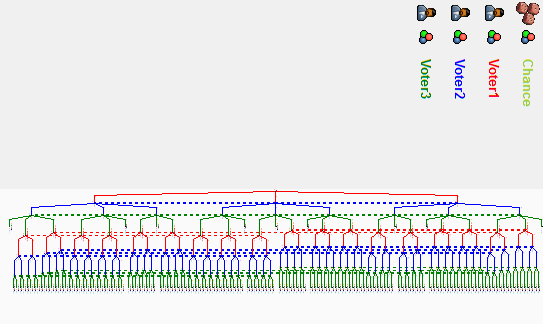
\includegraphics[height=7cm]{figures/voting_big.png}
\caption{A többfordulós szavazás extenzív alakja}
\end{center}
\end{figure}
A második feladatot nem sikerült megoldani, mivel az ágens kifutott a memóriából a normál alak óriási mérete miatt. Ezért egy egyszerűbb szavazó sémát hoztam létre, ami csak egy fordulóból állt, 3 szavazó és 3 jelöltel.
\begin{figure}[h]
\begin{center}
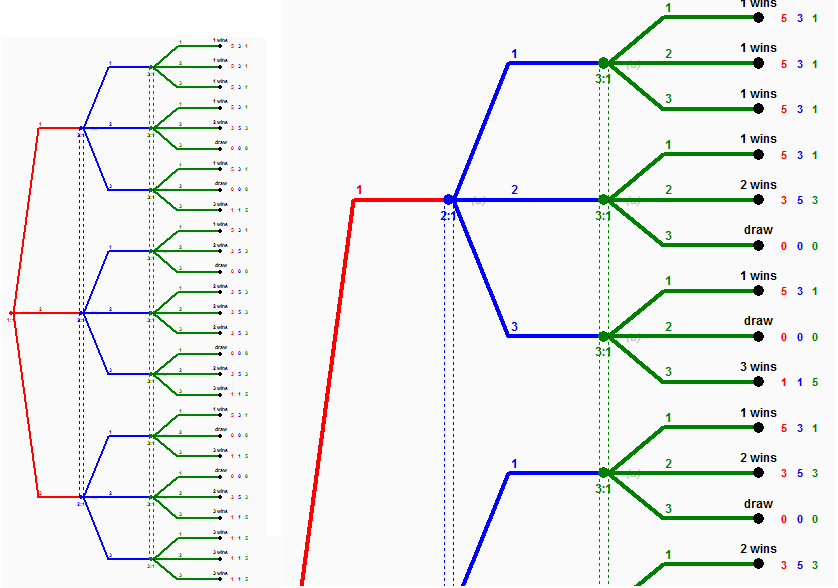
\includegraphics[height=7cm]{figures/voting_small.png}
\caption{Az egyfordulós szavazás extenzív alakja}
\end{center}
\end{figure}
\begin{figure}[h]
\begin{center}
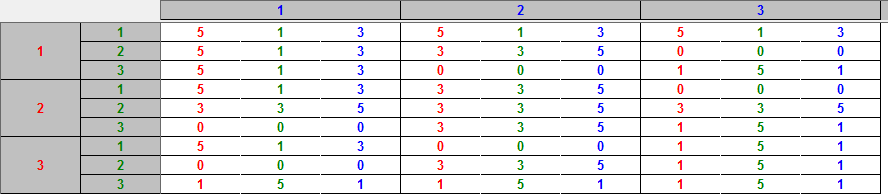
\includegraphics[height=5cm]{figures/voting_small2.png}
\caption{Az egyfordulós szavazás normál alakja}
\end{center}
\end{figure}
A leírt szavazó játéknak nincs domináns stratégiája és jópár Nash egyensúlya van.

\section{Labor feladat 2}
\subsection{Leírás}
Az 1-es feladatban kapott normál alakot adja meg a JADE-es játékvezető (msclab01.lab04.GameAgent), és néhány gépi játékos ágens (msclab01.lab04.PlayerAgent) számára, majd végezzen velük kísérleteket! Milyen lejátszások adódnak a játékosok különböző beállításai (pl. stratégia-választó programja) mellett? Elérhető-e, illetve stabil-e a Nash-egyensúly? Mi a legjobb stratégia/program (ha pl. UserAgent ágenssel játszunk adott gépi ágensek, vagy akár más hallgatók által vezérelt UserAgent ágensek ellen)? 
\subsection{Megoldás}
Az előbb definiált játékot futtatva a JADEX platformon a következő eredményt kaptam.
\begin{lstlisting}[caption=Szavazás run config, frame=single,float=!ht]
-container -port 1099 -host localhost 
ga:msclab01.gametheory_lab.GameAgent.GameAgent(voting_game 3 3) 
pa0:jadex.adapter.jade.JadeAgentAdapter(msclab01.gametheory_lab.PlayerAgent.Player 
"default gid=\\\"voting_game\\\" gui=true myType=7") 
pa1:jadex.adapter.jade.JadeAgentAdapter(msclab01.gametheory_lab.PlayerAgent.Player 
"default gid=\\\"voting_game\\\" gui=true myType=7")
pa2:jadex.adapter.jade.JadeAgentAdapter(msclab01.gametheory_lab.PlayerAgent.Player 
"default gid=\\\"voting_game\\\" gui=true myType=7")
\end{lstlisting}
\begin{figure}[h]
\begin{center}
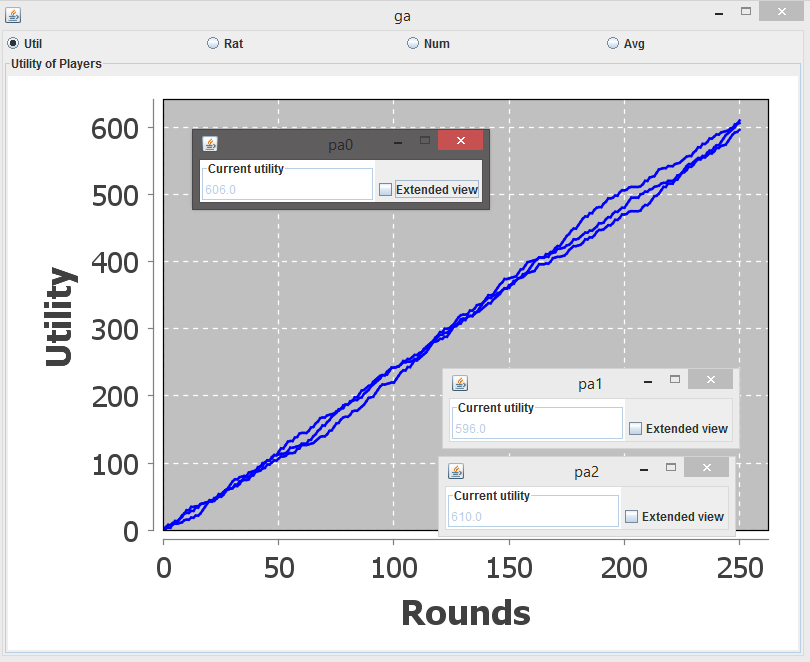
\includegraphics[height=7cm]{figures/voting_jadex.png}
\caption{Ágens szavazó játékeredmény}
\end{center}
\end{figure}

\section{Labor feladat 3}
\subsection{Leírás}
Alakítsa ki GAMBIT-ben egy legalább 3 szereplős, legfeljebb néhány lépésből álló egyszerűbb aukció (pl. angol, holland, vagy japán aukció) extenzív alakját, majd konvertálja ezt át normál alakba, elemezze, és mentse a games könyvtárba! Ellenőrizze az elkészült játékot az msclab01.gametheory-lab.Game osztály segítségével is! 
\subsection{Megoldás}
A létrehozott aukció játéknak 3 játékosa lehet, egy termékre licitálnak és 2 pénzel rendelkeznek. A termék valós értéke 4, tehát ha egy játékos megveszi 1 ért, akkor a haszna 3.
Komplexebb aukció leírását sajnos most sem sikerült a JADEX platformon futtatni.
\begin{figure}[h]
\begin{center}
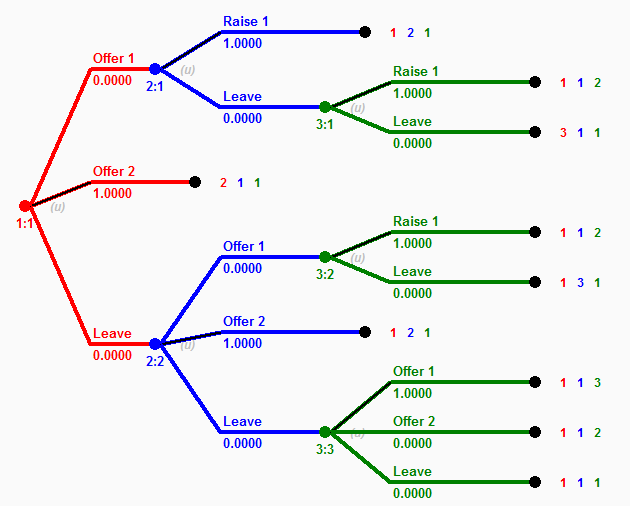
\includegraphics[height=7cm]{figures/auction.png}
\caption{Az aukció játék extenzív alakja}
\end{center}
\end{figure}


\section{Labor feladat 4}
\subsection{Leírás}A 3-as feladatban kapott normál alakot adja meg egy JADE-es GameAgent játékvezető és néhány Player gépi játékos ágens számára, majd végezzen velük kísérleteket! Milyen lejátszások adódnak a játékosok különböző beállításai (pl. stratégia-választó programja) mellett? Elérhető-e, illetve stabil-e a Nash-egyensúly? Mi a legjobb stratégia/program (ha pl. UserAgent ágenssel játszunk adott gépi ágensek, vagy akár más hallgatók által vezérelt UserAgent ágensek ellen)?   
\subsection{Megoldás}
A létrehozott aukció játékot JADEX ágensekkel lejátszva a következő eredményt kaptam. A stratégiák változtatása nem járt különösebb eredményel, hisz a játék csak egy lépéses.
\begin{lstlisting}[caption=Aukció run config, frame=single,float=!ht]
-container -port 1099 -host localhost 
ga:msclab01.gametheory_lab.GameAgent.GameAgent(auction_game 3 3) 
pa0:jadex.adapter.jade.JadeAgentAdapter(msclab01.gametheory_lab.PlayerAgent.Player 
"default gid=\\\"auction_game\\\" gui=true myType=7") 
pa1:jadex.adapter.jade.JadeAgentAdapter(msclab01.gametheory_lab.PlayerAgent.Player 
"default gid=\\\"auction_game\\\" gui=true myType=7")
pa2:jadex.adapter.jade.JadeAgentAdapter(msclab01.gametheory_lab.PlayerAgent.Player 
"default gid=\\\"auction_game\\\" gui=true myType=7")
\end{lstlisting}
\begin{figure}[!h]
\begin{center}
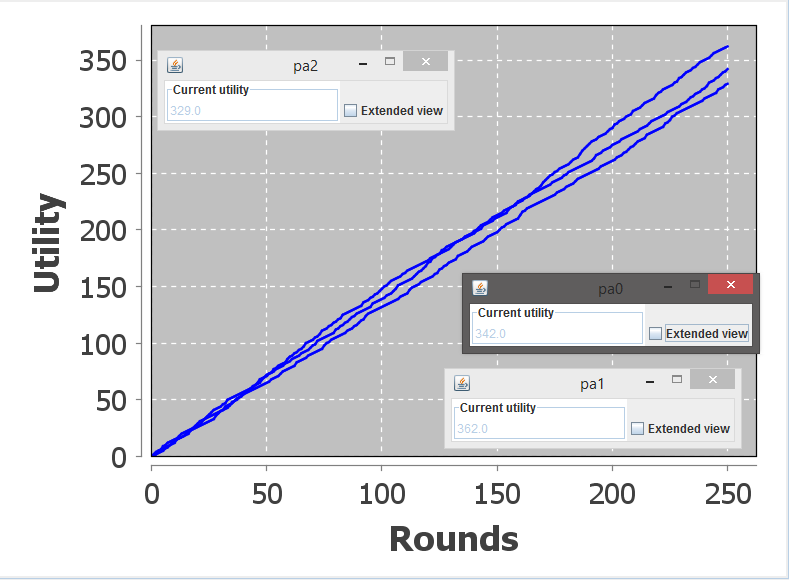
\includegraphics[height=7cm]{figures/auction_jadex.png}
\caption{Ágens aukció játékeredmény}
\end{center}
\end{figure}
\section{Összefoglalás}
A labor során megismerkedtem a játékok GAMBIT-al való leírásával, megoldásával. Ez követően szimulációkat végeztem JADEX ágensekkel, akik lejátszották az adott játékokat. Tapasztaltam hogy a játékok világában a leírás exponenciálisan nő a játékosok, lehetséges lépések számával. Kis lépésszám melett a GAMBIT alkalmas volt a játék modellezésére, de nagy lépésszámnál a Nash egyensúly számolás és domináns stratégia keresés már sikertelen volt.